% !TeX program = lualatex
% !TeX encoding = utf8
% !TeX spellcheck = uk_UA
% !TeX root =../MexPractEng.tex

%=========================================================
\chapter{Universal Gravitation. Central-force problem}\label{\currfilebase}
\Opensolutionfile{answer}[\currfilebase/\currfilebase-Answers]
\Writetofile{answer}{\protect\section*{\nameref*{\currfilebase}}}%
%=========================================================


%=========================================================
\begin{problem}\label{prb:cfp_three_bodyes}
	\addpic{2}{0.4\linewidth}{%
	\begin{tikzpicture}
		\pgfmathsetmacro{\R}{0.3}
		\draw[-latex] (-1,0) -- +(5.5,0) node[right] {$x$};
		\draw[-latex] (0,-1) -- +(0,5) node[above] {$y$};
		\coordinate (A) at (0,3); 
		\coordinate (B) at (0,0); 
		\coordinate (C) at (3.5,0); 
		\draw let \p{A} = (A), \p{B} = (B) in (\x{A}, \y{A}) -- +(-1,0);
		\draw[latex-latex] let \p{A} = (A), \p{B} = (B) in  ({\x{A} - 0.6cm}, \y{A}) -- node[left] {$d_1$} ({\x{A} - 0.6cm}, \y{B});		
		\draw let \p{C} = (C) in (\x{C},0) -- +(0,-1);
		\draw[latex-latex] let \p{C} = (C), \p{B} = (B) in  (0, {\y{B} - 0.6cm}) -- node[below] {$d_2$} (\x{C} , {\y{B} - 0.6cm});
		\foreach \i in {A,B,C} {
			\fill[ball color = orange!50] (\i) node[] {\i} circle (\R);
		}
	\end{tikzpicture}
	\captionof{figure}{Problem~\ref{prb:cfp_three_bodyes}}
	\label{cfp_three_bodyes}
	}
	In Fig.~\ref{cfp_three_bodyes}, three $5.00$~kg spheres are located at distances $d_1  = 0.300$~m and $d_2 = 0.400$~m. What are the 
	\begin{enumerate*}[label=(\alph*)]
		\item magnitude 
		and 
		\item direction (relative to the positive direction of the $x$ axis) of the net gravitational force on sphere B due to spheres A and C?
		\item What is the gravitational potential energy of the system?
	\end{enumerate*}
\end{problem}

%=========================================================
\begin{problem}
	\correct{0.4\linewidth}[7]%
	Planet Roton, with a mass about of $7.0 \cdot 10^{24}$~kg and a radius of $1600$~km, gravitationally attracts a meteorite that is initially at rest relative to the planet, at a distance great enough to take as infinite. The meteorite falls toward the planet. Assuming the planet is airless, find the speed of the meteorite when it reaches the planet's surface.
	\begin{solution}
		$2.4 \cdot 10^4$~\si{\meter\per\second}.
	\end{solution}
\end{problem}

%=========================================================
\begin{problem}
	%\correct[5ex]{0.4\linewidth}[3]
	Consider a pulsar, a collapsed star of extremely high density, with a mass $M$ equal to that of the Sun ($1.98 \cdot 10^{30}$~kg), a radius $R$ of only $12$~km, and a rotational period $T$ of $0.041$~s. By what percentage does the free-fall acceleration differ from the gravitational acceleration at the equator of this spherical star?
	\begin{solution}
		$0.03\%$.
	\end{solution}
\end{problem}


%=========================================================
\begin{problem}
	A projectile is fired vertically from Earth’s surface with an initial speed of $10$~km/s. Neglecting air drag, how far above the surface of Earth will it go?
	\begin{solution}
		$2.5 \cdot 10^4$~\si{\kilo\meter}.
	\end{solution}
\end{problem}


%=========================================================
\begin{problem}\label{prb:cfp_least_ke}
	Figure~\ref{cfp_U(r)} gives the potential energy function $U(r)$ of a projectile, plotted outward from the surface of a planet of radius $R_s$. 
	\begin{enumerate*}[label=(\alph*)]
		\item What least kinetic energy is required of a projectile launched at the surface if the projectile is to <<escape>> the planet?
		If the projectile is launched radially outward from the surface with a mechanical energy of $-2.0 \cdot 10^9$~\si{\joule}, what are
		\item its kinetic energy at radius $r = 2R_s$ 
		and
		\item its turning point in terms of $R_s$?
	\end{enumerate*}

	\begin{solution}
		\begin{enumerate*}[label=(\alph*)]
			\item $5.0 = 10^9$~\si{\joule};
			\item $0.5 = 10^9$~\si{\joule};
			\item $3.5R_s$.
		\end{enumerate*}
	\end{solution}
\end{problem}


%=========================================================
\begin{problem}\label{prb:cfp_ke_asteroid}
	Figure~\ref{cfp_ke_asteroid} is a graph of the kinetic energy $K$ of an asteroid
	versus its distance $r$ from Earth’s center, as the asteroid falls directly
	in toward that center. 
	\begin{enumerate*}[label=(\alph*)]
		\item What is the (approximate) mass of
		the asteroid?
		\item What is its speed at $r = 1.945 \cdot 10^7$~m?
	\end{enumerate*}
	\begin{solution}
		\begin{enumerate*}[label=(\alph*)]
			\item $1.0 \cdot 10^3$~kg; 
			\item $1.5$~km/s.
		\end{enumerate*}
	\end{solution}
\end{problem}

%=========================================================
\begin{figure}[h!]\centering
	%---------------------------------------------------------
	\begin{minipage}[t]{0.47\linewidth}\centering
	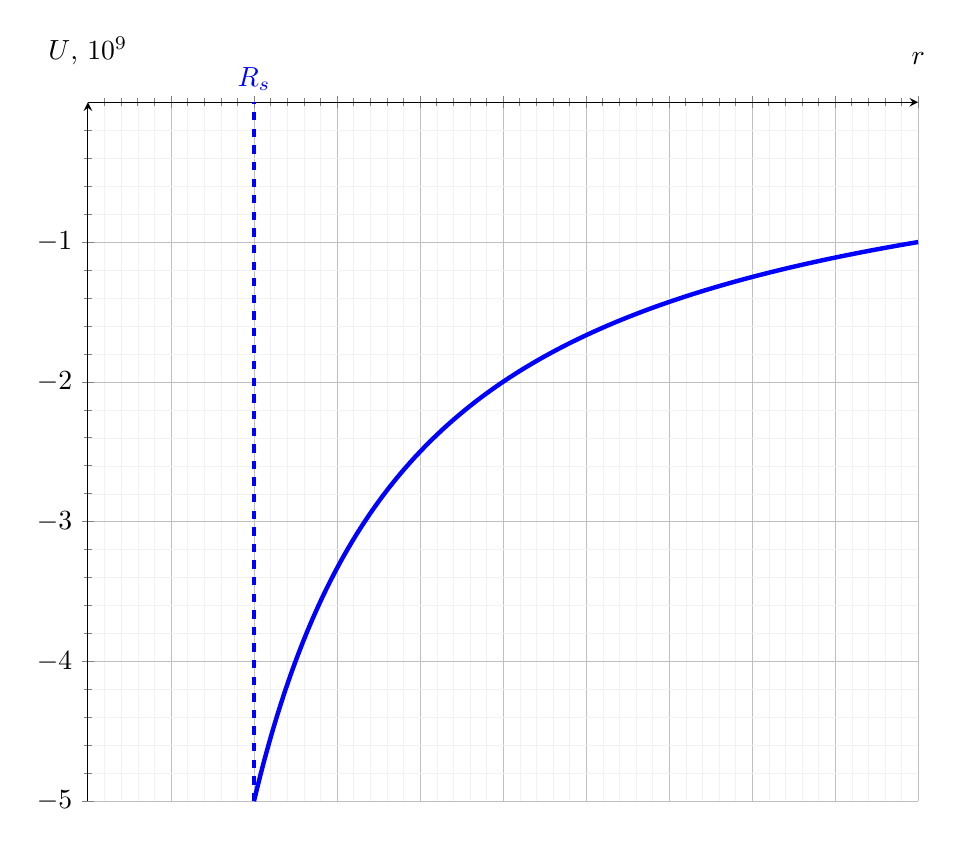
\begin{tikzpicture}[baseline]
		\begin{axis}[%
		clip = false, 
		% === Налаштування сітки ===
		grid = both,
		grid style={line width=.1pt, draw=gray!10},
		major grid style={line width=.2pt,draw=gray!50},
		minor tick num = 4,
		minor grid style = {line width=.1pt,draw=gray!10},
		% === Налаштування положення координатних осей ===
		axis lines = middle,
		axis line style={-stealth},
		% === Вибір підписів шкали для відображення ===
		xticklabels={},
		ytick = {-5,...,0},
		% === Підпис координатних осей ===
		xlabel={$r$},
		ylabel={$U$, $10^9$ \si{\joule}},
		% === Положення підпису координатних осей ===
		xlabel style={above = 10pt},
		ylabel style={above = 10pt},
		% === Налаштування мінімальних та максимальних значень координат ===
		xmin = 0,
		xmax =  1,
		ymin = -5,
		ymax =  0,
		% === Налаштування розміру графіка ===
		width=\linewidth,
		]
		\addplot+[blue, no marks, domain={0.2:1}, samples=500, ultra thick] {-1/x};
		\addplot+[dashed, blue, no marks, ultra thick] coordinates {(0.2, -5) (0.2, 0)} node[above] {$R_s$};
		\node[below, text=white] at (0.2, -5) {1};
		\end{axis}
	\end{tikzpicture}
	\caption{Problem~\ref{prb:cfp_least_ke}}
	\label{cfp_U(r)}
	\end{minipage}
	%---------------------------------------------------------
	\begin{minipage}[t]{0.47\linewidth}\centering
	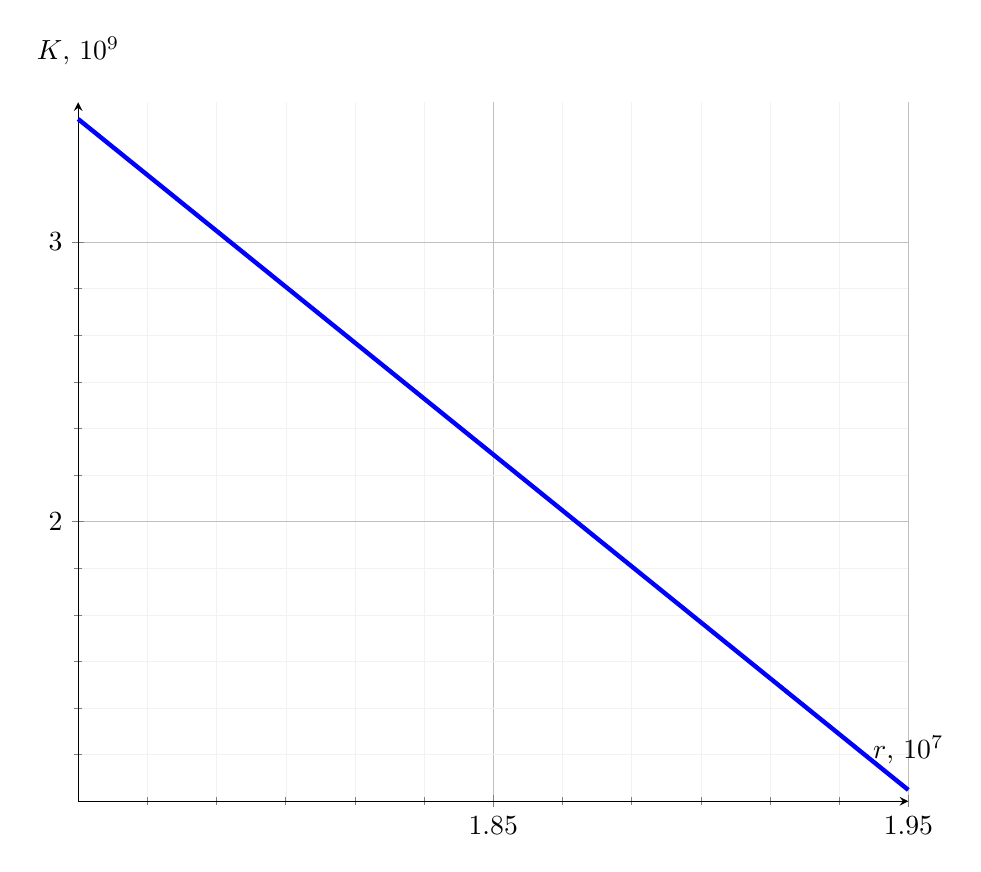
\begin{tikzpicture}[baseline]
		\begin{axis}[%
		clip = false, 
		% === Налаштування сітки ===
		grid = both,
		grid style={line width=.1pt, draw=gray!10},
		major grid style={line width=.2pt,draw=gray!50},
		minor tick num = 5,
		minor grid style = {line width=.1pt,draw=gray!10},
		% === Налаштування положення координатних осей ===
		axis lines = middle,
		axis line style={-stealth},
		% === Вибір підписів шкали для відображення ===
		xtick={1.75,1.85,1.95},
		ytick = {1,2,3},
		% === Підпис координатних осей ===
		xlabel={$r$, $10^7$ \si{\meter} },
		ylabel={$K$, $10^9$ \si{\joule}},
		% === Положення підпису координатних осей ===
		xlabel style={above = 10pt},
		ylabel style={above = 10pt},
		% === Налаштування мінімальних та максимальних значень координат ===
		xmin = 1.75,
		xmax =  1.95,
		ymin = 1,
		ymax =  3.5,
		% === Налаштування розміру графіка ===
		width=\linewidth,
		]
		\addplot+[blue, no marks, domain={1.75:1.95}, samples=100, ultra thick] {-12*x+24.44};
		\end{axis}
	\end{tikzpicture}
	\caption{Problem~\ref{prb:cfp_ke_asteroid}}
	\label{cfp_ke_asteroid}
	\end{minipage}
	%---------------------------------------------------------
\end{figure}
%=========================================================



%=========================================================
\begin{problem}
	In a binary star system, two stars follow circular orbits
	about their common center of mass. If the stars have masses $m_1$ and
	and $m_2$ are separated by a distance $r$, show that the period of rotation
	is related to $r$ by
	\[
		T^2  = \frac{4\pi^2 r^3}{G(m_1 + m_2)}.
	\]
\end{problem}


%=========================================================
\begin{problem}
	Using the conservation laws, demonstrate that the total 
	mechanical energy of a planet of mass $m$ moving around the Sun 
	along an ellipse depends only on its semi-major axis $a$. Find this 
	energy as a function of $a$. 
	\begin{solution}
		$E = - G\frac{Mm}{2a}$, where $M$ is the mass of the Sun. 		
	\end{solution}
\end{problem}


%=========================================================
\begin{problem}
	A double star is a system of two stars moving around the 
	centre of inertia of the system due to gravitation. Find the distance 
	between the components of the double star, if its total mass equals $M$ 
	and the period of revolution $T$. 
	\begin{solution}
		$\sqrt[3]{GM\left(\nfrac{T}{2\pi}\right)^2}$.
	\end{solution}
\end{problem}


%=========================================================
\begin{problem}\label{prb:cfp_four_stars}
	A certain quaternary star system consists of three stars,
	each of mass $m$, moving in the same circular orbit of radius
	$r$ about a central star of mass $M$. The stars orbit in the same
	sense and are positioned one-third of a revolution apart
	from one another (Fig.~\ref{cfp_four_stars}). Derive an expression for the period of revolution of the stars.
	\begin{solution}
		$T = \frac{2\pi r ^{\nfrac32}}{\sqrt{G(M + \nfrac{m}{\sqrt3})}}$.
	\end{solution}
\end{problem}


%=========================================================
\begin{problem}\label{prb:cfp_triple_star}
	A certain triple-star system consists of two stars, each of mass $m$, revolving in the same circular orbit of radius $r$ around a central star of mass $M$ (Fig.~\ref{cfp_triple_star}). The two orbiting stars are always at opposite ends of a diameter of the orbit. Derive an expression for the period of revolution of the stars.
	\begin{solution}
		$T = \frac{2\pi r ^{\nfrac32}}{\sqrt{G(M + \nfrac{m}{4})}}$.
	\end{solution}
\end{problem}

%=========================================================
\begin{figure}[h!]\centering
	%---------------------------------------------------------
	\begin{minipage}[t]{0.45\linewidth}\centering
	\begin{tikzpicture}
		\pgfmathsetmacro{\R}{2}
		\draw[dashed, cyan, rotate=45,
		postaction=decorate, 
		decoration={markings, 
			mark= at position 0.25 with 
			{\arrow{latex};},
			mark= at position 0.75 with 
			{\arrow{latex};}	
		},
		] (0,0) circle (\R);
		\fill[ball color = red!50] (0,0) circle (0.5);
		\foreach \i in {1,2,3} {
		\coordinate (B\i) at ({120*\i-30}:\R);
		\fill[ball color = orange!50] (B\i) circle (0.2);
		}
		\draw[-latex] (0,0) -- node[fill=white] {$r$} +(90:\R);
		\end{tikzpicture}
		\captionof{figure}{Problem~\ref{prb:cfp_four_stars}}
		\label{cfp_four_stars}
	\end{minipage}
	%---------------------------------------------------------
	\begin{minipage}[t]{0.45\linewidth}\centering
	\begin{tikzpicture}
		\pgfmathsetmacro{\R}{2}
		\draw[dashed, cyan, rotate=45,
		postaction=decorate, 
		decoration={markings, 
			mark= at position 0.25 with 
			{\arrow{latex};},
			mark= at position 0.75 with 
			{\arrow{latex};}	
		},
		] (0,0) circle (\R);
		\fill[ball color = red!50] (0,0) circle (0.5);
		\draw[rotate=45] (-\R,0) coordinate (B1)  (0,0)  (\R,0) coordinate (B2);
		\fill[ball color = orange!50] (B1) circle (0.2);
		\fill[ball color = orange!50] (B2) circle (0.2);
		\draw[-latex] (0,0) -- node[fill=white] {$r$} +(90:\R);
		\end{tikzpicture}
		\captionof{figure}{Problem~\ref{prb:cfp_triple_star}}
		\label{cfp_triple_star}
	\end{minipage}
	%---------------------------------------------------------
\end{figure}
%=========================================================



%=========================================================
\begin{problem}
	A $50$~kg satellite circles planet Cruton every $6.0$~h.The magnitude
	of the gravitational force exerted on the satellite by Cruton is
	$80$~N. 
	\begin{enumerate*}[label=(\alph*)]
		\item What is the radius of the orbit?
		\item What is the kinetic energy of the satellite?
		\item What is the mass of planet Cruton?
	\end{enumerate*}
\end{problem}



%=========================================================
\begin{problem}\label{prb:cfp_ir1.210}
	\addpic{2}{0.3\linewidth}{%
		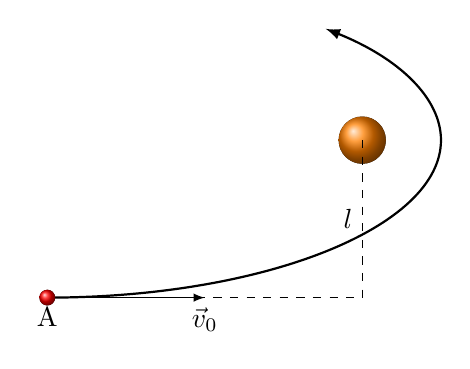
\begin{tikzpicture}
		\draw[-latex, thick] (0,0) +(-90:5 and 2) coordinate (A) arc (-90:45:5 and 2); 
		\fill[ball color = orange] (4,0) circle (0.3);
		\draw[-latex] (A) -- +(2,0) node[below] {$\vec v_0$};
		\draw[dashed] (A) -- ({A-|4,0});
		\draw[dashed] (4,0) -- node[left] {$l$} ({A-|4,0}) ;
		\fill[ball color = red] (A) node[below] {A} circle (0.1);
		\end{tikzpicture}
		\captionof{figure}{Problem~\ref{prb:cfp_ir1.210}}
		\label{cfp_ir1.210}
	}
	A cosmic body A moves to the Sun with velocity $v_0$ (when 
	far from the Sun) and aiming parameter $l$ the arm of the vector $\vec v_0$ 
	relative to the centre of the Sun (Fig.~\ref{cfp_ir1.210}). Find the minimum  
	distance by which this body will get to the Sun. 
	\begin{solution}
		$r_{\min} = G\frac{M}{v_0^2}\left( \sqrt{1+ \left(\frac{lv_0^2}{GM}\right)^2 } - 1\right) $, where $M$ --- is the mass of Sun.
	\end{solution}
\end{problem}

%=========================================================
\begin{problem}
	\correct{0.3\linewidth}[4]%
	Comet Halley moves about the Sun in an elliptical orbit, with its closest approach to the Sun being about $0.590$ AU and its greatest distance $35.0$~AU ($1$ AU is the Earth–Sun distance). The comet’s speed at closest approach is $54.0$~km/s. What is its speed when it is farthest from the Sun?
	\begin{solution}
		$0.910$~\si{\kilo\meter\per\second}.
	\end{solution}
\end{problem}




\Closesolutionfile{answer}

